

%%%%%%%%%%%%%%%%%%%%% LateX template %%%%%%%%%%%%%%%%%


%%%%%%%%%%%% inicio del documento incluyendo opciones %%%%%%%%%%%%%%%%%%%%%%%%%%%%%%%
\documentclass[letterpaper,11pt]{article}
%%%%%%%%%%%%%%%%%%%%%%%%%%%%%%%%%%%%%%%%%%%%%%%%%%%%%%%%%%%%%%%%%%%%%%%%%%%%

%%%%%%% paquetes utiles: español, incluir graficos, etc %%%%%%%%%%%%%%%%%%%%%%%%%%%%
\usepackage[utf8]{inputenc}
\usepackage{amsmath}
\usepackage{amsfonts}
\usepackage{amssymb}
\usepackage{amsthm}
\usepackage[spanish]{babel}
\usepackage{latexsym}
\usepackage{euscript}
\usepackage{graphicx}
\usepackage{tdclock}
\usepackage{subcaption} 
%%%%%%%%%%%%%%%%%%%%%%%%%%%%%%%%%%%%%%%%%%%%%%%%%%%%%%%%%%%%%%%%%%%%%%%%%%%%%%%%%%

%%%%%%%%%%%%%%%%%%% espacio para la primera linea del parrafo %%%%%%%%%%%%%%%
\setlength{\parindent}{0mm} 
%%%%%%%%%%%%%%%%%%%%%%%%%%%%%%%%%%%%%%%%%%%%%%%%%%%%%%%%%%%%%%%%%%%%%%%%%%

%%%%%%%%%%%%%%% espacio entre parrafos %%%%%%%%%%%%%%%%%%%%%%%%%%%%%%%
\setlength{\parskip}{2mm}
%%%%%%%%%%%%%%%%%%%%%%%%%%%%%%%%%%%%%%%%%%%%%%%%%%%%%%%%%%%%%%%%%%%%

%%%%%%%%%%%%%%%%%%%%% espaciado entre lineas %%%%%%%%%%%%%%%%%%%%%%%%%%%%%
\linespread{1} 
%%%%%%%%%%%%%%%%%%%%%%%%%%%%%%%%%%%%%%%%%%%%%%%%%%%%%%%%%%%%%%%%%%%%%%

%%%%%%%%%%%%%%%%%%%%%%%% Control de margenes %%%%%%%%%%%%%%%%%%%%%%%%%%%%
%\setlength{\topmargin}{-1.cm}
\setlength{\oddsidemargin}{-.8cm}
\setlength{\evensidemargin}{-.8cm}
\setlength{\textheight}{24cm} 
\setlength{\textwidth}{18cm} 
\setlength{\headsep}{-2cm}
%%%%%%%%%%%%%%%%%%%%%%%%%%%%%%%%%%%%%%%%%%%%%%%%%%%%%%%%%%%%%%%%%%%%%%%%%%%%

%%%%%%%%%%%%%%%  definicion de comandos que se utilicen frecuentemente %%%%%%%%%%%%%%%
\def\und#1{\underline{#1}}
\def\be{\begin{equation}}
\def\ee{\end{equation}}
\def\bea{\begin{eqnarray}}
\def\eea{\end{eqnarray}}
%%%%%%%%%%%%%%%%%%%%%%%%%%%%%%%%%%%%%%%%%%%%%%%%%%%%%%%%%%%%%%%%%%%%%%%%%%%%%%%%%%%%
%%%%%%%%%%%%%%%%%%%%%%%%%%%%%%%%%%%%%%%%%%%%%%%%%%%%%%%%%%%%%%%%%%%%%%%%%%%%%%%%%%%%
\makeatletter 
\newcommand{\pder}[2]{\begingroup 
  \@tempswafalse\toks@={}\count@=\z@ 
  \@for\next:=#2\do 
    {\expandafter\check@var\next\@nil
     \advance\count@\der@exp 
     \if@tempswa 
       \toks@=\expandafter{\the\toks@\,}% 
     \else 
       \@tempswatrue 
     \fi 
     \toks@=\expandafter{\the\expandafter\toks@\expandafter\partial\der@var}}% 
  \frac{\partial\ifnum\count@=\@ne\else^{\number\count@}\fi#1}{\the\toks@}% 
  \endgroup} 
\def\check@var{\@ifstar{\mult@var}{\one@var}} 
\def\mult@var#1#2\@nil{\def\der@var{#2^{#1}}\def\der@exp{#1}} 
\def\one@var#1\@nil{\def\der@var{#1}\chardef\der@exp\@ne} 
\makeatother

\makeatletter 
\newcommand{\der}[2]{\begingroup 
  \@tempswafalse\toks@={}\count@=\z@ 
  \@for\next:=#2\do 
    {\expandafter\check@var\next\@nil
     \advance\count@\der@exp 
     \if@tempswa 
       \toks@=\expandafter{\the\toks@\,}% 
     \else 
       \@tempswatrue 
     \fi 
     \toks@=\expandafter{\the\expandafter\toks@\expandafter d \der@var}}% 
  \frac{d \ifnum\count@=\@ne\else^{\number\count@}\fi#1}{\the\toks@}% 
  \endgroup} 
\def\check@var{\@ifstar{\mult@var}{\one@var}} 
\def\mult@var#1#2\@nil{\def\der@var{#2^{#1}}\def\der@exp{#1}} 
\def\one@var#1\@nil{\def\der@var{#1}\chardef\der@exp\@ne} 
\makeatother

\begin{document}

\begin{center}
{\bf \Large Juego de monedas} 
\end{center}

\noindent
{\bf \large Carlos Manuel Rodríguez Martínez} \hspace{5.2cm} {\bf \large Fecha: 21/04/2015} 

\smallskip

\section*{Caminante aleatorio (juego de las monedas)}
El juego consiste en que un número $N$ de jugadores tira una moneda $M$ veces. Los jugadores comienzan con una cantidad inicial de monedas $m_0$. Se escoge una cara de la moneda como la ganadora, y otra cara como la perdedora. Si al tirar la moneda el jugador obtiene la cara ganadora, gana una moneda. Si obtiene la cara perdedora, pierda una moneda. El juego termina cuando el jugador se queda sin dinero.

\subsection*{Análisis analítico}
Si se ve el número de monedas como una posición espacial, el juego consiste en dar $n$ pasos con longitud igual $a$ a la izquerda o la derecha. Después de $n$ pasos la posición $x$ a la que se llega es
\[
	x = a \left(S-(n-S) \right) = a(2S-n),
\]
donde $S$ es el número de pasos a la derecha. Entonces
\[
	S = \frac{x}{2a}+\frac{a}{2}.
\]
Sea $\tau$ el tiempo que toma dar un paso, el tiempo total es $t = n \tau$.

Luego, hay $n \choose s$ maneras distintas de dar $S$ pasos a la derecha de un total de $n$. La probabilidad de dar $S$ pasos a la derecha de un total de $n$ es
\[
	P(S,n) = {n \choose s} \left( \frac{1}{2} \right)^n,
\]
entonces
\[
	P(x,t) = {\frac{t}{\tau} \choose \frac{t}{2 \tau} + \frac{x}{2a}} \left( \frac{1}{2} \right)^n,
\]
esto es la probabilidad de llegar al punto $x$ en un tiempo $t$. Para el caso cuando $n$ y $s$ son grandes podemos usar la fórmula de Stirling y hacer aproximaciones. El resultado es
\[
	f(x,t) = (2 \pi D)^{-\frac{1}{2}} e^{- \frac{x^2}{2 D t}},
\]
siendo $f(x,t) = \frac{1}{2a} P(x,t)$ y $D = \frac{a^2}{\tau}$. $f(x,t)$ es la densidad de probabilidad que nos da la probabilidad de que a tiempo $t$ el caminante esté en el intervalo $x$, $x+dx$.
Entonces se espera que al hacer el juego con un número grande de jugadores se obtenga una distribución normal.

\subsection*{Análisis de la simulación}
Se realizó una simulación en la que se implementa el juego de la moneda. Fue implementada utilizando el lenguaje de programación C++ debido a la necesidad de un alto rendimiento al hacer pruebas con un número grande de jugadores. Para la generación de números aleatorios se utilizó el algoritmo \textit{Mersenne-Twister}.

La primera prueba se realizó con un número de jugadores $N=500000$, tirando la moneda $M=15$ veces y una cantidad inicial de monedas $m_0 = 15$. Los resultados de esta simulación se muestran en la figura \ref{fig:Juego1}.
\begin{figure}[h!]
\begin{subfigure}{.5\textwidth}
	\centering
	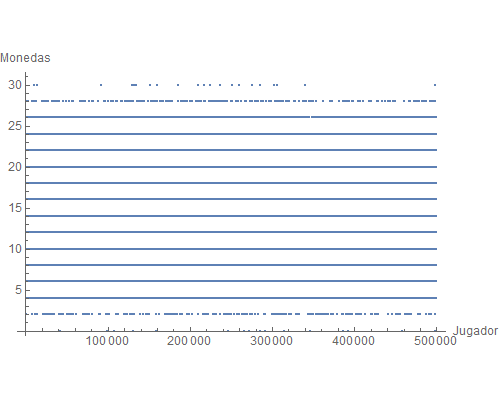
\includegraphics[scale=0.5]{img/Fig6}
	\caption{Número de monedas de cada jugador.}
\end{subfigure}%
\begin{subfigure}{.5\textwidth}
	\centering
	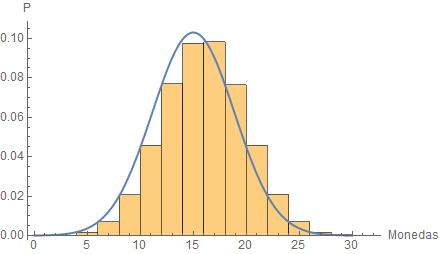
\includegraphics[scale=0.5]{img/Fig1}
	\caption{Distribución de monedas.}
\end{subfigure}%
\caption{Primer juego.}
\label{fig:Juego1}
\end{figure}
Se ajustó una curva de distribución normal sobre el histograma de frecuencias, dando como resultado una distribución con media de $\mu = 15.001$ y varianza $\sigma^2 = 3.87201$. Esto es congruente con el análisis analítico.

Al realizar el juego con la cantidad inicial de monedas $m_0 = 15$ se está haciendo que se pueda caminar libremente sin que exista una dirección preferencial. El juego cambia cuando se escoge una cantidad inicial de monedas más cercana al cero. Por ejemplo, al hacer el juego con $m_0 = 1$ la mitad de los jugadores perderán en el primer turno, haciendo que ya no puedan seguir y acumulándose en el cero, como se muestra en la figura \ref{fig:Juego2}.
\begin{figure}[h!]
\begin{subfigure}{.5\textwidth}
	\centering
	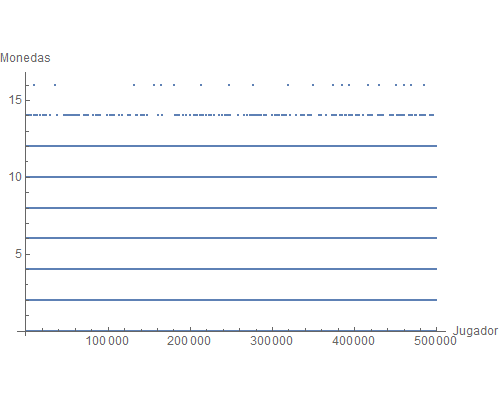
\includegraphics[scale=0.5]{img/Fig2}
	\caption{Número de monedas de cada jugador.}
\end{subfigure}%
\begin{subfigure}{.5\textwidth}
	\centering
	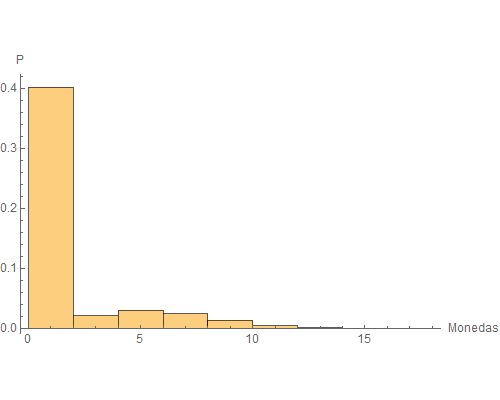
\includegraphics[scale=0.5]{img/Fig4}
	\caption{Distribución de monedas.}
\end{subfigure}%
\caption{Segundo juego.}
\label{fig:Juego2}
\end{figure}
La distribución no sigue una ley de potencias. Esto se ve en la figura \ref{fig:LogLog}, en la que se hace un ajuste de la gráfica Log-Log del histograma de ocurrencias.
\begin{figure}[h!]
\centering
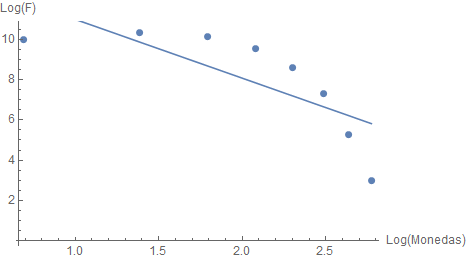
\includegraphics[scale=0.55]{img/Fig3}
\caption{Ajuste de gráfica Log-Log.}
\label{fig:LogLog}
\end{figure}
Llama la atención que si bien el primer máximo está en cero, como cabría esperar, el segundo máximo no está adyacente al cero, sino más lejos. Esto ocurre sin importar la cantidad de jugadores o lanzamientos de monedas. Para ilustrar el motivo de este comportamiento se hará el análisis de la distribución de monedas. Supongamos que $m_0 = 1$, y $x_n$ es el porcentaje de jugadores con $n$ monedas. En el primer turno
\[
	x_0 = 0, \quad x_1 = 1, \quad x_2 = 0, \cdots,
\]
en el segundo turno la mitad pierde la moneda, la otra mitad gana. Entonces
\[
	x_0 = \frac{1}{2}, \quad x_1 = 0, \quad x_2 = \frac{1}{2}, \cdots,
\]
en el tercero
\[
	x_0 = \frac{1}{2}, \quad x_1 = \frac{1}{4}, \quad x_2 = 0, \quad x_3 = \frac{1}{4} \cdots,
\]
en el cuarto
\[
	x_0 = \frac{5}{8}, \quad x_1 = 0, \quad x_2 = \frac{1}{4}, \quad x_3 = 0, \quad x_4 = \frac{1}{8} \cdots.
\]
Haciendo una lista con todos los porcentajes de cada turno da como resultado
\begin{align*}
&\{0,1\},\left\{\frac{1}{2},0,\frac{1}{2}\right\},\left\{\frac{1}{2},\frac{1}{4},0,\frac{1}{4}\right\},\left\{\frac{5}{8},0,\frac{1}{4},0,\frac{1}{8}\right\},\left\{\frac{5}{8},\frac{1}{8},0,\frac{3}{16},0,\frac{1}{16}\right\},\left\{\frac{11}{16},0,\frac{5}{32},0,\frac{1}{8},0,\frac{1}{32}\right\},\\
&\left\{\frac{11}{16},\frac{5}{64},0,\frac{9}{64},0,\frac{5}{64},0,\frac{1}{64}\right\},\left\{\frac{93}{128},0,\frac{7}{64},0,\frac{7}{64},0,\frac{3}{64},0,\frac{1}{128}\right\},\left\{\frac{93}{128},\frac{7}{128},0,\frac{7}{64},0,\frac{5}{64},0,\frac{7}{256},0,\frac{1}{256}\right\}, \\
&\left\{\frac{193}{256},0,\frac{21}{256},0,\frac{3}{32},0,\frac{27}{512},0,\frac{1}{64},0,\frac{1}{512}\right\},\left\{\frac{193}{256},\frac{21}{512},0,\frac{45}{512},0,\frac{75}{1024},0,\frac{35}{1024},0,\frac{9}{1024},0,\frac{1}{1024}\right\}, \cdots.
\end{align*}
Esto se puede visualizar mejor utilizando un mapa de colores y coloreando cada valor fraccional en cada paso, esto se muestra en la figura \ref{fig:AC}.
\begin{figure}[h!]
\centering
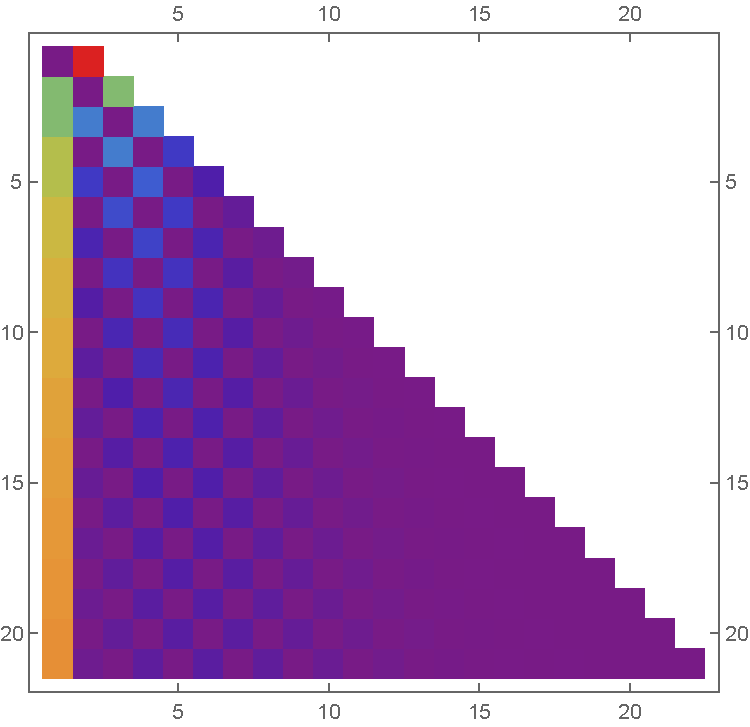
\includegraphics[scale=0.6]{img/Fig7}
\caption{Fracción de jugadores en cada punto.}
\label{fig:AC}
\end{figure}
En esta figura el eje vertical representa la iteración del juego, y el eje horizontal representa los $x_n$. Este resultado tiene cierta similitud con un autómata celular, y muestra cómo es que se distribuyen los jugadores haciendo que el segundo máximo esté alejado del cero.

\end{document}
